\documentclass{standalone}
\usepackage{tikz}
\usetikzlibrary{shapes.geometric,arrows.meta,babel,positioning}
\tikzset{%
    >={Latex[width=2mm,length=2mm]},
    base/.style = {
        rectangle, rounded corners, draw=black, minimum width=4cm,
        minimum height=1cm, text centered, font=\sffamily
    },
    startLoop/.style = {base, fill=blue!30},
    process/.style = {
        base, minimum width=2.5cm, fill=orange!15, font=\ttfamily
    },
}
\begin{document}
    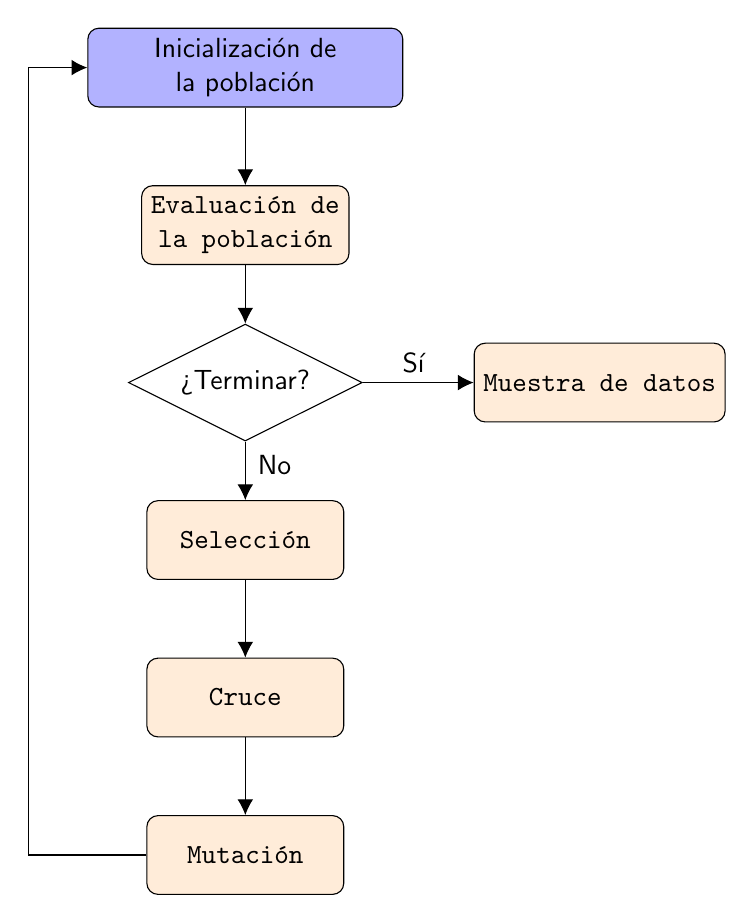
\begin{tikzpicture}[
        node distance=1.5cm,
        every node/.style={fill=white, font=\sffamily},
        align=center
    ]
        % Nodes position
        \node (start)         [startLoop]
                                {Inicialización de\\la población};
        \node (evaluate)       [process, below of=start, yshift=-0.5cm]
                                {Evaluación de\\la población};
        \node (finish)      [
                draw, diamond, aspect=2, below of=evaluate, yshift=-0.5cm
        ] {¿Terminar?};
        
        \node (showResults)      [process, right of=finish, xshift=3cm]
            {Muestra de datos};

        \node (selection) [process, below of=finish, yshift=-0.5cm]
                                {Selección};
        \node (crossover)  [process, below of=selection, yshift=-0.5cm]
                                {Cruce};
        \node (mutation)        [process, below of=crossover, yshift=-0.5cm]
                                {Mutación};
        % Arrow specification
        \draw[->]         (start) -- (evaluate);
        \draw[->]       (evaluate) -- (finish);
        \draw[->] (finish) -- node[right,xshift=1,yshift=2]{No}(selection);
        \draw[->] (finish) -- node[anchor=south,above]{Sí} (showResults);
        \draw[->]  (selection) -- (crossover);
        \draw[->]  (crossover) -- (mutation);
        \draw[->] (mutation.west) -- ++(-1.5, 0) -- ++(0,10) -- (start.west);
    \end{tikzpicture}
\end{document}